\chapter{Analysis of Twitter's Social Structure}


Stuff to add to this section:
\begin{itemize}
\item Change tweet features for each simulation and make comparison on these differences
\item Observe differences in patterns when network generation parameters are altered
\item Link up section to previous section (i.e. how did the previous research help and how does this build on that work?)
\item Explain how this section becomes the basis for work in 'main chapter 3'.
\item (e.g. Issues with current method (too long, requires network, inaccurate due to having to choose users with fewer followers), so need a quicker, more accessible and online approach).
\item Explain the Mechanical Turk questions in more detail, with examples.
\item Discuss about the machine learning approach used (logistic regression and how it works)
\item Link 'retweet volume' to 'retweet group size'
\end{itemize}


In the previous chapter, a series of studies were conducted into Twitter with respect to message propagation through retweeting. In particular, research was done to provide an understanding of the patterns produced through retweets and how their properties relate to the Twitter users that the Tweets pass through.

Of particular interest, however, is the social graph underlying Twitter, which describes how the users are interconnected and dictates the information flow between them. It has been discussed that users with a higher follower count are more likely to have their Tweets retweeted and that some users can have their Tweets forwarded through many hops indeed, so that information may be passed between different communities of users.

In addition to the effects of user influence,  several other factors also govern an individual retweet decision of a given user for a particular Tweet. These include properties of the Tweet, such as whether, or not, the Tweet contains a URL, whether it mentions a particular user, whether the user even has an opportunity to view the Tweet, and so on.\\
These factors account for the individual user's retweet decision and the almagamation of every user's retweet decision on the Tweet describes the Tweet's overall retweetability and, which determines how far the Tweet can propagate.

However, it is believed that the topology of the network, below the level of user influence, can play an important role in facilitating (or inhibiting) Tweet propagation by opening and closing available retweet pathways between users and groups of users.\\
Whilst retweet decisions based on Tweet features alone (such as the actual content of the Tweet or a URL the Tweet points to) may imply a level of interest in the Tweet, the influence of users has a very large impact on how many retweets a certain Tweet receives. Thus, abstracting the concepts away from user influence may help in discovering methods for inferring which information is interesting.

Twitter's social structure has previously been described as being built from users creating edges between themselves through the act of following. A followship defines the direction of travel of information from the follower to the friend, and this illustrates how users with many followers immediately have their Tweets made available to lots of users before any retweeting even takes place.\\
As more edges are constructed between users, then the global initial spread of Tweets is increased, and with the addition of retweets, this has an even bigger effect. Although other infleuncing factors have been mentioned earlier, such as the notion of a user's network awareness and of user influence, the organisation of users on the graph and the differences in observed propagation pattern is an interesting avenue for research towards uncovering interestingness.

In this chapter, various user network types are used to simulate retweet behaviour between users on Twitter. The behaviours are studied in order to research the propagation patterns observed in different network structure types. Non-realistic and realistic networks are used to highlight the low-level propagation in these networks and the similarities between more realistic simulated networks and Twitter's own social graph.\\
This research is then used to generate the methodology for estimating Tweet interestingness based on an \textit{expected} Tweet popularity, as is discussed further later in the chapter.


\section{Observing Differences in Propagation Patterns Between Different Network Structures}
In this section, simulations are carried out in three different network topologies - a path (or `linear') network, a random network, and a scale-free network. In the experiments, individual user \textit{decisions} are used as the bases for demonstrating Tweeting and retweeting.  

The simulation algorithm and ideas behind the model used for generating the simulated users' retweet decisions are adapted from the work carried out in \cite{zhu11} and \cite{peng11}, which introduces methodologies for illustrating Tweet spread through a given network of users.\\
From the analyses of the simulation experiments, of interest is whether, and how, changing the network structure does affect retweet propagation patterns, and whether a simulation can mimic Twitter's own bhevaiour in terms of retweet spread.

Measuring retweet behaviour is carried out through studying the distribution of retweet group sizes that result from running the experiments, as is described in later sections.


\subsection{Overview of the Simulation Algorithm}
The algorithm covers the simulation of Tweet propagation through a given set of connected users by emulating retweet decisions of each user who receives the Tweet. The retweet decision is made based on a logistic regression, as is described later.

\cite{zhu11} developed a simulation algorithm which carried this out, which was found to work accurately. This algorithm was modified to fit the purposes of the experiments in this section.\\
In essence, the simulation initially requires a graph of connected users, $U$, and a Tweet, $t$, to be retweeted between them. It begins by initialising a set of users, $S$, to contain the followers of a particular $u_s \in U$, which represents the user $t.\textrm{author}_O$. As such, users in $S$ are the current set of users to have $t$ on their home timeline.\\
The procedure then iterates over timesteps, at each stage checking the retweet probability of each $u \in S$. If $u$'s retweet probability is suffuciently great for $t$, then $u$ retweets $t$ by being removed from $S$ and then added to $RT(t)$, which represents the set of users who have retweeted $t$. The followers of $u$ are then added to $S$.\\
A threshold value, $TH$, is used to emulate the idea of Tweet `decay'. The reasoning behind this is that as time goes by, more and more Tweets arrive onto the home timeline, pushing the previous Tweets further down, whether they are interesting or not. Tweets may be ignored and not retweeted if the user has not viewed their home timeline for a while or if the user decides the Tweet is not of a sufficient quality to retweet it. If a Tweet is pushed down to the extent that is out of view, or out of the current page, then the chance of that user retweeting that Tweet is reduced. Thus, if a user is in $S$ for more iterations than specified by $TH$, then the user is removed from $S$, meaning they cannot retweet the Tweet.\\
Users who have retweeted $t$, or are unable to do so (either by having previously retweeted it or by exceeding $TH$) are prevented from being (re-)added to $S$.

The algorithm terminates either when the timesteps exceed the maximum allowed, $T$, or when $S$ becomes empty. This results in the retweet group, $G(t)$, which comprises the final set, $RT(t)$, along with the initial $u_s$. As in the previous chapter, $t.\textrm{count}_R = |RT(t)|$.

Therfore, the additional necessary components to run the simulation are the functionality to build the user graph, a constructed Tweet, and functionality for generating a retweet probability for each user who receives the Tweet.

\newfloat{algorithm}{H}{lop}
\begin{algorithm}
\caption{Simulation of retweet decisions in a given network of users}
\begin{algorithmic}[1]
\Procedure{simulate}{graph of users $U$, tweet $t$}
    \State $RT\gets$ empty set \Comment{To hold users who retweet $t$}
    \State $T\gets$ number of timesteps allowed
    \State $TH\gets$ maximum timesteps \Comment{Emulate $t$ `slipping' down timeline}
    \State $us\gets$ source User selected from $U$
    \State $S\gets$ initialise to followers of $us$
    \Statex % new line
    \ForAll{$ti$ in range $(0,T)$}
        \ForAll{$u \in S$}
            \State $P\gets$ retweet probability of $u$ on $t$ in range $(0,1)$
            \State $r\gets$ random number in range $(0,1)$
            \If{$P > r$}
                \State Remove $u$ from $S$
                \State Add $u$ to $RT$
                \State Add followers of $u$ to $S$
            \Else
                \State increment $u.\textrm{TIME\_HELD}$
                \If{$u.\textrm{TIME\_HELD} > TH$}
                    \State remove $u$ from $S$ \Comment{$u$ has held $t$ for too long in timeline}
                \EndIf
            \EndIf
        \EndFor
        \If{$|S| = 0$}
            \State return $RT$ \Comment{No more users can retweet $t$}
        \EndIf
    \EndFor
    \State return $RT$
\EndProcedure
\end{algorithmic}
%\caption{Algorithm to simulate retweet decisions in a given network of users.}
\label{algo1}
\end{algorithm}


\subsection{Generating a User's Retweet Probability} 
As prevoiusly mentioned, \cite{zhu11} used a predictive model for retweet decisions based on a logistic regression, which was demonstrated to be capable of accurately predicting a user's retweet chance on a given Tweet at a given time. The regression was trained on a set of user, tweet and context features in order to classify a likelihood on the binary decision: retweet or no retweet, such that if $P = 1$ then the retweet will definitely occur.


\subsubsection{Machine Learning}
Machine learning is the term given to the family of techniques that allow a program to make predictions for the outcome of unseen instances based on an observed and known history of occurrences. There are many types of machine learning classifiers that are suitable for different purposes, such as for predicting an expected outcome from a set of nominal categories, for predicting a value from a continuous range, or for predicting the \textit{probability} of a binary outcome.

Most machine learning techniques involve the training of a predictive model, which contains the information on known outcomes for a set of features. The model is then used to estimate an unknown outcome, usually with a probability on the \textit{confidence} of the classification, for new sets of instances.

For example, consider three attribute variables, $A$, $B$, and $C$, each of which can be equal to one of two nominal values; \textsc{True} or \textsc{False}. A particular machine learning algorithm trains a model based on its knowledge that;
\begin{itemize}
    \item $A\gets$ \textsc{True}, $B\gets$ \textsc{False} $\Longrightarrow$ $C\gets$ \textsc{True}
    \item $A\gets$ \textsc{False}, $B\gets$ \textsc{False} $\Longrightarrow$ $C\gets$ \textsc{False}
\end{itemize}
Although training of predictive models nearly always involves using more than two instances, the history of these example instances indicate that $C$ is more strongly associated with $A$ than with $B$. As more instances are added showing similar behaviours, then the association becomes stronger, to the extent that the technique will predict $C\gets$ \textsc{True} in instances where $A\gets$ \textsc{True} (and vice versa) with higher confidence.

In this case, $A$, $B$, and $C$ are known as the `features', and a set of such features form the `instance'. Once a trained model has been constructed, the machine learning algorithm will only be able to make predictions using instance features it has knowledge of. For example, if the example technique was now given an instance containing a feature $D$, then the example technique will not know how changes in $D$ will affect $C$'s outcome.

If there is not a strong correlation between the features in a dataset, then the confidence on classification of a particular feature will be weaker. Although this example has focussed on boolean (nominal) data types, many machine learning classifiers are able to work with features that are higher dimensional nominal values, contunuous reals, and so on, and will apply weights to the different features based on their level of influence to other features in the instance.


\subsubsection{The Logistic Regression}
Logistic regression analysis can be used as a machine learning technique for working with binary outcomes based on a set of predictor variables (or features) \cite{hosmer13}, which makes it an appropriate approach for predicting the binary retweet decision. As mentioned previously, logistic regressions have been frequently used in retweet analysis \cite{castillo11} \cite{zhu11} \cite{peng11} \cite{naveed11} \cite{hong11}.

An implementation of the logistic regression algorithm was written in the Python programming language, which formed the basis of calculating the value for $P$ mentioned in the algorithm overview earlier based on a set of feautures of the Tweet and author user.


\subsection{Summary of Training Features}
\cite{zhu11} used the approach in order to accurately model retweet decisions in Twitter. A set of around 50 different features were used to train the logistic regression, with the retweet outcome (\textsc{True} or \textsc{False}) being the predicted classification in each case. These features included tweet-related features (such as content analysis, inclusion of URLs, etc.), and network and user features (followships, mentions, etc.).

Since the network structures themselves, and the propagation \textit{patterns}, are what are of interest in this section, the simulation is significantly simplified by using far fewer features, yet which are features that have been shown to have a strong influence on the retweet decision. As long as a consistent set of feature groups and values are used, the properties of the retweet groups observed should demonstrate the varying behaviours across the different user structures.

As such, each instance comprised the following four features associated with each Tweet, $t$, and where $u$ is the user currently making the retweet decision, \textsc{retweet};

\begin{table}[h]\footnotesize
\begin{center}
\begin{tabular}{ l | c | l }
	Feature & Data type & Description\\
	\hline
	\hline 
	\textsc{follows}    & \{\textsc{True, False}\} & \textsc{True} if $u \in t.\textrm{author}_O.E_i$\\
    \textsc{followed}   & \{\textsc{True, False}\} & \textsc{True} if $u \in t.\textrm{author}_O.E_o$\\
    \textsc{mentioned}  & \{\textsc{True, False}\} & \textsc{True} if $u$ is mentioned in $t$'s content\\
    \textsc{url}        & \{\textsc{True, False}\} & \textsc{True} if \texttt{http://} or \texttt{https://} in $t$'s content\\
    \hline 
    \textsc{retweet}    & \{\textsc{True, False}\} & \textsc{True} if $u \in RT(t)$\\ 
    \hline
\end{tabular}
\end{center}
\caption{Training features for the logistic regression.}
\label{table:logisticregressionfeatures}
\end{table}

The \textsc{url} feature has, in the literature, often been found as a large impacting feature on retweets in Twitter, especially in \cite{alonso10}, who use it as their basis for determining which Tweets are interesting.


\subsection{Training the Model}
In order to train the logistic regression model, data was required from Twitter so that the instance sets of features could be built. 

Data collection for these experiments again utilised Twitter's REST API, which was queried between March and June 2012 to collect a set of around 12,000 Tweets and retweets. Since this time was before the mandatory switch-over to v1.1 of the REST API, the public timeline could again be used to collect the data without the necessity of crawling through the social graph.\\
In this case, it was particularly necessary that non-retweets were also collected in order to provide the negative case when training the regression model, so that there were instances where the \textsc{retweet} feature could be \textsc{False}.

In cases where the collected Tweet was a retweet, further calls were made to the API to determine the relationships between the retweet's author and the original Tweet's author in order to satisfy the required \textsc{follows} and \textsc{followed} features.
Where the collected Tweet was not an instance of retweet, there is no original author to examine the relationships between. In these cases, further Tweets were retrieved for the user in order to find their retweet rate in terms of the ratio of retweets to Tweets on their user timeline and an analysis of the relationship between these and the original authors. This was used in conjunction with the user's follower and friend count to determine a probability of the `faux' followships.

After storage, the regression model was trained using features extracted from the raw data, which the simulation algorithm could then use to generate the required retweet probability, $P$.


\subsection{Running the Simulations}
Once the model had been trained, the simulations could be run. In each simulation experiment, a network of users was generated, as described in the next section, and a Tweet object was created.\\
This Tweet object contained information on whether or not it contained a URL and if it mentioned one of the users in the generated network. 

Various parameters - such as the $TH$, the size of the user network, $U$ to be generated, $t$'s particular parameter for the simulation, and any weightings on the decision probability prediction generator - could be altered to affect the strength or correlation of the patterns produced by the different network structure types.


\subsection{Network Analyses}
In this section, three network structures are assessed in terms of the differences in the patterns of propagation each expresses. Each generated graph is a \textit{directed} graph in order to illustrate the followships between the user nodes, and to support the use of the \textsc{follows} and \textsc{followed} features required in the decision probability calculation.

In each case, the same set of generated Tweets were used, but different structures required the various parameters to be set slightly differently.


\subsubsection{Path Network}
The first assessed structure was to illustrate the pattern on a non-realistic social network structure; a path network.

Path networks are one of the simplest type of graph, and a linear directional path network consists of the graph of users, $U$, of size $n$, in which each user $U_i \forall 0 \leq i < n$ is followed by user $U_{i+1}$. As a result, each $u \in U$ has precisely one follower and one friend, except the users $U_n$ and $U_1$ respectively.

\begin{figure}[h]
\centering
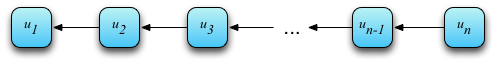
\includegraphics[scale=0.8]{4.Chapter2/Media/path_network.png} 
\caption{Example of a path network.}
\label{fig:path_network}
\end{figure}

In this graph, the size of the retweet group is, by definition, equal to the depth of penetration, as there is only one path (or retweet chain) available for propagation to occur down. As such, in each case, the retweet tree representing a resultant retweet group formed in this type of network will have the same structure as the graph itself, yet with a size dependent on the collective retweet decisions of the users.

Since each internal user has only one follower, the likelihood of a retweet decision being positive at each timestep is somewhat progressively reduced, and thus is much more likely to tail off sooner than in graphs with more propagation avenues. This is also due to the fact that each retweet can only reach an audience of size 1 at each time step, and thus the survival of the retweet cannot rely on a summation of many users' retweet decisions. 

\begin{figure}[h]
\centering
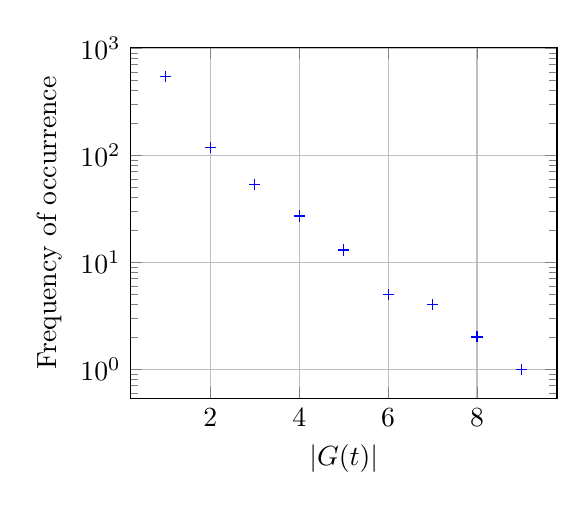
\begin{tikzpicture}
 \begin{semilogyaxis}[
        xlabel=$|G(t)|$,
        ylabel=Frequency of occurrence,
        width=7cm,
        grid = major]
    \addplot[only marks,mark=+,blue] plot coordinates {
        (1,540)  (2,118)  (3,53) (4,27) (5,13) (6,5) (7,4) (8,2) (9,1) (10,0)
    };
\end{semilogyaxis}
\end{tikzpicture}
\caption{Frequency distribution of retweet group sizes in path network simulations}
\label{fig:linear}
\end{figure}

The likelihood of a particular user achieving the opportunity to receive the Tweet, in order to then retweet it, becomes the product of the probability function the further it travels through the graph, in which user $U_i$ requires each user from $U_{i-1}$ to first make a positive retweet decision. For example, if each user has probability $p$ of retweeting the Tweet, then each user's chance of retweeting the Tweet is $\frac{1}{p^i}$, where $i$ is the position of the user in the graph.

Therefore, as might be expected, the frequency distribution of retweet group sizes demonstrates a logarithmic pattern with many small retweet groups followed by a series of exponentially smaller groups.



As a result, if the retweet decision chance of each user is more or less equal, the chance of user $ N_2  $ retweeting the tweet is of an order of magnitude less than that of user $ N_1 $ deciding to retweet. The graph shows half life-style behaviour; owing to the fact that each retweet is exponentially less likely to occur than the previous retweet. Note that the graph is plotted on a log-linear scale.

- This network illustrates well how some users who might find the tweet interesting (and then retweet the Tweet) do not even get to see it in order to make the decision

\subsubsection{Random Network}
Random networks are more similar to Twitter's own social structure than path networks, but are a much more basic and uniform version and do not consider more influential users or the development of Twitter communities.
\\
A random network is defined as a network of users, $ N $, of size $ n $ in which a user $ N_x $ has probability $ p $ of following user $ N_y $. Thus; as the probability $ p $ is increased, the likelihood of a user following other users in $ N $ increases, causing the overall network edge density to increase. Generally, the average number of followers and followees of a user is proportional to $ p\times n $. Thus the parameters for constructing such a graph are the network size, $n$, and the attachment probability, $p$. The simulation results for the random network indicates a higher distribution of mid-range retweet volumes.
\begin{figure}[h]
\centering{
\begin{tikzpicture}
 \begin{semilogyaxis}[
        xlabel=Retweet Volume,
        ylabel=Frequency,
        grid = major]
    \addplot[only marks,mark=*,blue]
       file {4.Chapter2/data/random.dat};    
\end{semilogyaxis}
\end{tikzpicture}
\caption{Retweet volume frequency distribution from random network simulation}
\label{fig:random}
}
\end{figure}

\subsubsection{Scale-Free Network}
Include more mathematical analysis of scale-free networks (in general) - i.e., in what way are they logarithmic?
\\
A scale-free network is a network of users, $ N $, of size $ n $ and is generated in such a way so that the resultant distribution of degree follows a power-law. \emph{In}-degree signifies the number of inward edges to a node (i.e. the number of followers of a user), whereas \emph{out}-degree is the number of outward edges (i.e. the number of users that user follows).
\\
Scale-free networks have been the subject of a fair amount of research, and are explained more thoroughly in \cite{hein06}. In our implementation we use NetworkX\footnote{http://networkx.lanl.gov}, a Python networking package, to generate directed scale-free networks through a preferential-attachment algorithm based on the network size and edge density as parameters.
\\
Figure \ref{fig:real-scalefree} shows the frequency distribution of retweet volumes. Since the data is plotted on logarithmic scales, we see a logarithmic trend very similar to our results in \cite{webberley11}.
%\begin{figure}[h]
%\centering{
%\begin{tikzpicture}
% \begin{loglogaxis}[
%        xlabel=Retweet Volume,
%        ylabel=Frequency,
%        grid = major]
%    \addplot[only marks,mark=*,blue]
%       file {data/scale-free.dat};
%    
%\end{loglogaxis}
%\end{tikzpicture}
%\caption{Retweet volume frequency distribution generated in scale-free networks}
%\label{fig:scale-free}
%}
%\end{figure}

\subsection{Comparison to Real Twitter Data}
In our previous work, \cite{webberley11}, we captured and analysed data which contained results on the distribution of retweet group sizes. In that paper, a retweet group was defined to be a set of tweets containing one tweet and then all the retweets of that tweet. Thus the retweet volume looked at in this section is effectively the cardinality of the retweet group (minus one). Since the results in the above experiments also look at the frequency distribution of retweet volumes, then we should be able to draw some comparisons.
\\
We compared the data produced by the different types of network to this previous data, and found that the scale-free network produced a distribution similar to that from the real Twitter data.
\begin{figure}[h]
\centering{
\begin{tikzpicture}
 \begin{loglogaxis}[
        xlabel=Retweet Volume,
        ylabel=Frequency,
        grid = major,
        legend entries={Real data,Scale-free}]
    \addplot[only marks,mark=*,red]
       file {4.Chapter2/data/comparison-real.dat};
    \addplot[only marks,mark=*,blue]
       file {4.Chapter2/data/comparison-scale-free.dat};
\end{loglogaxis}
\end{tikzpicture}
\caption{Comparing the retweet volumes distribution from scale-free graph simulation to data from Twitter's graph}
\label{fig:real-scalefree}
}
\end{figure}

\subsection{Structure Comparison}
Each network structure has been demonstrated to show different propagation characteristics. This has shown that, in addition to a user's own retweet decision, the actual spread of a tweet depends somewhat on how the author's local network is constructed. With lots of edges in the graph, there are many more paths down which propagation can occur, increasing the number of times a retweet decision is made, and therefore an increase in the overall number of retweets occurring. The retweet decision facilitated by the model, therefore, combined with a user network give an overall \textit{retweetability} of a tweet that will vary depending on the network it's being propagated in, the source user, and the intermediary retweeters.
\\
The path network, as designed to be the extreme case, has shown to allow poor propagation. Importantly, whilst the network parameters and retweet decision had to be globally increased to obtain any sensible data from this simulation, the trend still shows how propagation down a single chain isn't hugely effective.
\\
The random network facilitated many more retweets due to the fact that users had a very similar in- and out-degree in all cases across the network. This means that each user is able to receive a lot of information, and is also able to pass on (whether an author or a retweeter) information to lots of users simultaneously in the graph. 
\\ 
Despite random networks supporting large retweet throughput (i.e. high \emph{recall} of information), the disadvantage is that the interest \emph{precision}  is much lower. This is because this type of network relies on users following a large number of other users, thus meaning that they would receive more `noise' (i.e. uninteresting tweets) than if they were more limited and selective. Although tweets that are retweeted are usually of a higher \emph{quality}, not all retweeted tweets will be interesting to all users.
\\
Finally, the scale-free network, whilst not having the highest throughput of information, does have trends most similar to the data on retweet distributions collected from Twitter's social graph. This is due to its ability to emulate more influential users and areas of dense communities (as discussed in \cite{java07}). These networks have the potential to allow for large numbers of retweets, especially if they are sourced from one of these more dense areas, but typically die off more quickly as the tweets are retweeted through less influential users.


\section{Interesting Additional Findings}

\subsection{Graph Density}
Define edge density (with equation

\subsection{Results}
Show links between follower audience -> local network -> density.

\subsection{Uses}
From this data, it is demonstrable that various parameters can be generally successfully inferred from very basic user information.

\section{Predictions From the User Graph}
The final part of this paper focuses on the ongoing development of a method to predict the interestingness of a tweet based on the work in the previous sections. The prediction method, at a high level, compares the predicted retweet outcome of a given tweet to the number of times that tweet has actually been retweeted. If, for example, a tweet is simulated with the help of the model and produces a prediction of two retweets, but the tweet has actually been etweeted four times, then we can infer that this tweet is more interesting (at least, to a subset of users). 
\\
The tweet and user features we looked at earlier in this paper are very static, binary features, which do not take into account the actual content of the text of the tweet. Therefore, if a tweet is retweeted more than was predicted, then there is something in the tweet, such as a link to a particularly interesting article or a breaking news story, that makes it more interesting than the average tweet, with the same binary features, that was used to train the model.
\\
In order to improve the fairness of the experiment, we wanted to ensure that the environment of the tweets (i.e. the user network they are propagated through) is the same as its real-life Twitter counterpart. We could then choose a user, which would become the source user, $U_s$, in the set $U$, and simulate that user's own tweets within their particular local network as described by the model above. This would then produce a retweet volume for this user's tweets, to which we could compare the number of times that tweet has \emph{really} been retweeted.


\subsection{Data Collection}
Due to the exponential scaling properties of Twitter's social graph, it was infeasible to collect any more than two hops away from each user as a representation of that user's local network under the rate limitations of Twitter's REST API. 
\\
In particular, a single Twitter account running an instance of an application was allowed, at the time of these experiments, a maximum of 350 REST API calls per hour. One call would be required, for example, to obtain up to 5000 of the followers of a particular user (i.e. one follower hop from the user). An additional call would then be required to collect each of that user's follower's followers (in order to obtain the \emph{second} hop from the source user). \\
Thus, a user who has 700 followers would require 700 API calls to collect that follower network, in addition to the one required to collect that source user in the first place, and would therefore take over two hours of collection. To collect the \emph{third} hop from the source user would drastically multiply the number of required requests (even if there is significant overlap between the followers) and the time needed. 
\\
If each of the 700 followers of the source user had, on average, 200 followers, then this would require the gathering of $ 700 $ x $200 = 140,000 $ users, equating to more than 402 hours of data collection. Bearing in mind that this would only collect the network features for \emph{one} user, it is clear to see how this is an impractical approach.
\\ \\
Luckily, in \cite{webberley11}, we found that the vast majority of retweets occur \textit{within} two hops of the source user (i.e. a path length of less than three), so we considered that the distance from the source user in each case would be sufficient.
\\
In June 2012, the Twitter REST API was used to conduct a random walk through the social graph. For each user, we collected the most recent 300 tweets (including each tweet's metadata - particularly their retweet count) and their local follower network within two hops. We didn't collect the friend network, as we were only interested in tweets propagating outwards from the source user.
\\
After processing that user, the walker chose a user at random from the present user's set of followers and made this the new current user from which to collect data for. If the present user, at any stage, does not have any followers, a list of previously accepted users is maintained and a follower is chosen from one of those instead.
\\
The walker continued until the rate limit was met, at which time the current state was written to disk, and the walker waited until the rate limit was reset before continuing.
\\
Generally, this resulted in, for each user, a set of up to 300 tweets (totalling to around 10,000 tweets in total) and the network in which these tweets were propagated within. There was no need to collect any further data to train the regression, since we were able to re-use the trained model we used earlier.



\subsection{Validating Results}
Needed to validate results using human input. Machines themselves are generally unable to express human interests, so results need to be properly evaluated.

\subsubsection{Crowdsourcing}
Discuss crowdsourcing, its uses, how it is useful in this area. Talk about its history (with any references), and then about mechanical turk.
\\
Mention mechanics of mechanical turk, how it is US only (but we used crowdflower - which autmatically handles submission to MT and several other crowd-sourcing services.

\subsubsection{What We Wanted to Assess}
Used MK, etc.

\subsubsection{Constructing the Questions}
Set up questions (i.e. 5 tweets - choose most interesting and least interesting), give example of this.


In order to validate our prediction results, we ran a pilot user study in order to obtain some human input on the interestingness of each tweet. We compiled the tweet data into a set of questions which were submitted to Amazon's Mechanical Turk. Each question consisted of five tweets from our dataset and each Mechanical Turk Worker (MTW) undertook five questions. Each question asked the MTWs to select which tweet was the most interesting of the five, and which was the least interesting.
\\
For consistency we ensured that at least three MTWs had answered each question. When selecting tweets to include in the Mechanical Turk questions, we excluded those which are `@-replies' - i.e. tweets which begin with another user's screen-name and typically form part of a conversation between two or more users. This meant that there were around 4,500 tweets in total in the questions.

Through using the model and simulating each user's tweets through their individual local networks we achieved around 86\% accuracy in correctly predicting the number of times each tweet was retweeted. 
\\
The precision in predicting the \textit{interestingness} of each tweet was around 30\%. While this value is low, it does mean that in 30\% of cases, a tweet that we predicted to be interesting was verified to be interesting by at least three MTWs all selecting one tweet from a set of five. In addition, when simulating the questions by randomly choosing the most `interesting' tweet of the five in each case, the performance was unable to near our precision even after several thousand iterations.

\subsection{Improving This}
idea is there - need better idea for getting expected retweet value! problem is two-fold, but related - need too much data, and can only evaluate users with sparser local networks.
\\
Need offline methodology.
\\
One route for this would be to try and infer a user's local network from a set of their immediate parameters, drawing on our earlier work suggesting that the Twitter network has the properties of a scale-free small-world graph. Through studying graph patterns, it is possible to make sensible inferences on the edges and nodes of a user's local network based on their follower count. From this, a graph edge density can be calculated, $ d = \frac{|E|}{|N|(|N|-1)} $, for use in generating a scale-free network.
\\
Since, for these preliminary experiments, we were only able to collect data from users with a more modest local network, the real and predicted retweet values were both relatively low, allowing more room for error. When simulating much larger local networks involving many more real retweets for each tweet, predicting interestingness, with some threshold value, may become more accurate and thus help improve the precision. The reason for this is that the retweet count of tweets that naturally get retweeted many tens, hundreds, or more times is likely to vary more with interestingness than those that are naturally only retweeted very few times.

\section{Future Work}
There is much further research that could be carried out based on the results in this chapter. Now that the foundation has been laid for simple retweet prediction based on network analysis, research could begin to look at ways in which, as mentioned, networks could be generated based on a few environmental features surrounding users.
\\
This would allow for quick generation of user networks (bypassing the need for data collection) and would also support the same calculations for more highly influential users (users with more followers and more retweets per Tweet).
\\ \\
For this research, the notion of the network will continue and form the basis of the environmental features in the next chapter. Since we now know that the network plays an important role in dictating the way in which information can propagate

\section{Summary}
In this chapter we aimed to carry out a study on the behaviour of propagation through different types of social graph structures and to introduce our ongoing work into predicting the interestingness of tweets from their retweet patterns.
\\
Using a set of tweet and user features, we trained a regression model which we used to simulate a number of tweets through different network types. We produced a distribution of retweet volumes for each network type and confirmed that, with the same tweet features, different network configurations do indeed facilitate different retweet behaviours in terms of propagation spread. We were also able to compare our results to data from Twitter to verify that Twitter's own social graph most closely resembles a scale-free small world graph.
\\
We then finished by discussing how we used the trained model to simulate real networks from Twitter, along with the tweets that were passed through these networks, in order to try to predict how interesting a tweet is based on its retweet patterns. While we were able to often correctly predict the retweet outcome of a tweet, we found that more work would be required to improve the performance of predicting whether or not these tweets are truly interesting to users.
